\documentclass[letterpaper]{article}
\usepackage[margin=1in]{geometry}
\usepackage[utf8]{inputenc}
\usepackage{textcomp}
\usepackage{amssymb}
\usepackage{natbib}
\usepackage{graphicx}
\usepackage{gensymb}
\usepackage{amsthm, amsmath, mathtools}
\usepackage[dvipsnames]{xcolor}
\usepackage{enumerate}
\usepackage{mdframed}
\usepackage[most]{tcolorbox}
\usepackage{csquotes}
% https://tex.stackexchange.com/questions/13506/how-to-continue-the-framed-text-box-on-multiple-pages

\tcbuselibrary{theorems}

\newcommand{\R}{\mathbb{R}}
\newcommand{\Z}{\mathbb{Z}}
\newcommand{\N}{\mathbb{N}}
\newcommand{\Q}{\mathbb{Q}}
\newcommand{\C}{\mathbb{C}}
\newcommand{\code}[1]{\texttt{#1}}
\newcommand{\mdiamond}{$\diamondsuit$}
\newcommand{\PowerSet}{\mathcal{P}}
\newcommand{\Mod}[1]{\ (\mathrm{mod}\ #1)}
\DeclareMathOperator{\lcm}{lcm}

%\newtheorem*{theorem}{Theorem}
%\newtheorem*{definition}{Definition}
%\newtheorem*{corollary}{Corollary}
%\newtheorem*{lemma}{Lemma}
\newtheorem*{proposition}{Proposition}


\newtcbtheorem[number within=section]{theorem}{Theorem}
{colback=green!5,colframe=green!35!black,fonttitle=\bfseries}{th}

\newtcbtheorem[number within=section]{definition}{Definition}
{colback=blue!5,colframe=blue!35!black,fonttitle=\bfseries}{def}

\newtcbtheorem[number within=section]{corollary}{Corollary}
{colback=yellow!5,colframe=yellow!35!black,fonttitle=\bfseries}{cor}

\newtcbtheorem[number within=section]{lemma}{Lemma}
{colback=red!5,colframe=red!35!black,fonttitle=\bfseries}{lem}

\newtcbtheorem[number within=section]{example}{Example}
{colback=white!5,colframe=white!35!black,fonttitle=\bfseries}{def}

\newtcbtheorem[number within=section]{note}{Important Note}{
        enhanced,
        sharp corners,
        attach boxed title to top left={
            xshift=-1mm,
            yshift=-5mm,
            yshifttext=-1mm
        },
        top=1.5em,
        colback=white,
        colframe=black,
        fonttitle=\bfseries,
        boxed title style={
            sharp corners,
            size=small,
            colback=red!75!black,
            colframe=red!75!black,
        } 
    }{impnote}
\usepackage[utf8]{inputenc}
\usepackage[english]{babel}
\usepackage{fancyhdr}
\usepackage[hidelinks]{hyperref}

\pagestyle{fancy}
\fancyhf{}
\rhead{CSE 131}
\chead{Monday, April 03, 2023}
\lhead{Lecture 1}
\rfoot{\thepage}

\setlength{\parindent}{0pt}

\begin{document}

\section{Introduction to Compilers}
Some examples of compilers we've used in this class include 
\begin{center}
    \begin{tabular}{|c|c|}
        \hline 
        \code{gcc} & C to binary  \\ 
        \code{g++} & C++ to binary  \\ 
        \code{rustc} & Rust to binary \\ 
        \code{javac} & Java to JVM bytecode \\ 
        \code{ghc} & Haskell to Haskell magic \\ 
        \code{tsc} & TypeScript to JavaScript \\ 
        \hline 
    \end{tabular}
\end{center}
Essentially, a compiler takes some program and produces an output program, one that is easier for us to run in some environment. In this course, we're going to create a compiler \code{ucsdc} that takes in \code{snek} files and will produce \code{x86\_64} binaries.

\bigskip 

To be more specific, our compiler should do the following: given a \code{.snek} text file, 
\begin{itemize}
    \item parse\footnote{Known to be very boring.} the text into an abstract syntax tree (AST), 
    \begin{mdframed}
        (Example.) For example, consider the following Java class. 
\begin{verbatim}
class Pt {
    int x; 
    int y; 
}\end{verbatim}
        Its AST representation might look like 
        \begin{center}
            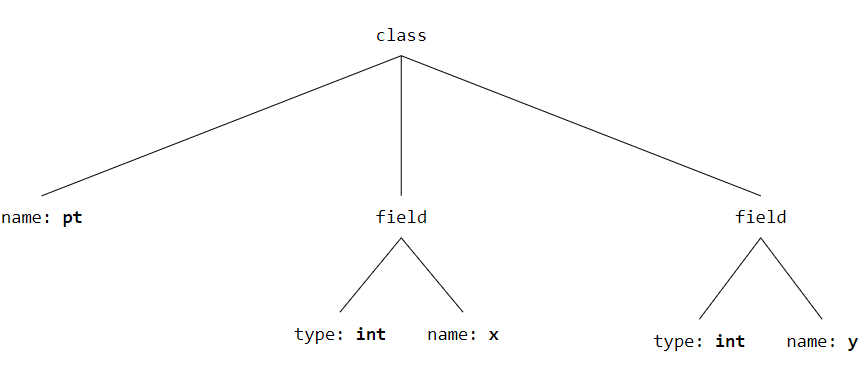
\includegraphics[scale=0.8]{../assets/ast.png}
        \end{center}
    \end{mdframed}
    \item and either 
    \begin{itemize}
        \item generates assembly (or some other output program), or 
        \item generate an error message.
    \end{itemize}
\end{itemize}
We are \underline{not} interested in generating the most optimized assembly, just that it works. Most of the time spent in this course will be on the code generating part (i.e., from AST to assembly). Towards the \emph{end} of the course, we'll work with libraries/runtime.

\subsection{Course Syllabus}
The course webpage can be found here: \href{https://ucsd-compilers-s23.github.io/index.html}{https://ucsd-compilers-s23.github.io/index.html}. 
\begin{itemize}
    \item Two exams during discussion (week 5, week 9).
    \item The final exam is skippable. The final exam can be used to improve your scores on the two exams. If you did well on the two exams, you don't need to do the final exam. 
    \item Engagement usually means weekly quiz on Gradescope and lecture handouts. They may help make the difference between an A and A+.
    \item Graduate students may be asked to do some additional things for the later projects.
\end{itemize}



\end{document}